% GNUPLOT: LaTeX picture with Postscript
\begingroup
  \makeatletter
  \providecommand\color[2][]{%
    \GenericError{(gnuplot) \space\space\space\@spaces}{%
      Package color not loaded in conjunction with
      terminal option `colourtext'%
    }{See the gnuplot documentation for explanation.%
    }{Either use 'blacktext' in gnuplot or load the package
      color.sty in LaTeX.}%
    \renewcommand\color[2][]{}%
  }%
  \providecommand\includegraphics[2][]{%
    \GenericError{(gnuplot) \space\space\space\@spaces}{%
      Package graphicx or graphics not loaded%
    }{See the gnuplot documentation for explanation.%
    }{The gnuplot epslatex terminal needs graphicx.sty or graphics.sty.}%
    \renewcommand\includegraphics[2][]{}%
  }%
  \providecommand\rotatebox[2]{#2}%
  \@ifundefined{ifGPcolor}{%
    \newif\ifGPcolor
    \GPcolortrue
  }{}%
  \@ifundefined{ifGPblacktext}{%
    \newif\ifGPblacktext
    \GPblacktexttrue
  }{}%
  % define a \g@addto@macro without @ in the name:
  \let\gplgaddtomacro\g@addto@macro
  % define empty templates for all commands taking text:
  \gdef\gplbacktext{}%
  \gdef\gplfronttext{}%
  \makeatother
  \ifGPblacktext
    % no textcolor at all
    \def\colorrgb#1{}%
    \def\colorgray#1{}%
  \else
    % gray or color?
    \ifGPcolor
      \def\colorrgb#1{\color[rgb]{#1}}%
      \def\colorgray#1{\color[gray]{#1}}%
      \expandafter\def\csname LTw\endcsname{\color{white}}%
      \expandafter\def\csname LTb\endcsname{\color{black}}%
      \expandafter\def\csname LTa\endcsname{\color{black}}%
      \expandafter\def\csname LT0\endcsname{\color[rgb]{1,0,0}}%
      \expandafter\def\csname LT1\endcsname{\color[rgb]{0,1,0}}%
      \expandafter\def\csname LT2\endcsname{\color[rgb]{0,0,1}}%
      \expandafter\def\csname LT3\endcsname{\color[rgb]{1,0,1}}%
      \expandafter\def\csname LT4\endcsname{\color[rgb]{0,1,1}}%
      \expandafter\def\csname LT5\endcsname{\color[rgb]{1,1,0}}%
      \expandafter\def\csname LT6\endcsname{\color[rgb]{0,0,0}}%
      \expandafter\def\csname LT7\endcsname{\color[rgb]{1,0.3,0}}%
      \expandafter\def\csname LT8\endcsname{\color[rgb]{0.5,0.5,0.5}}%
    \else
      % gray
      \def\colorrgb#1{\color{black}}%
      \def\colorgray#1{\color[gray]{#1}}%
      \expandafter\def\csname LTw\endcsname{\color{white}}%
      \expandafter\def\csname LTb\endcsname{\color{black}}%
      \expandafter\def\csname LTa\endcsname{\color{black}}%
      \expandafter\def\csname LT0\endcsname{\color{black}}%
      \expandafter\def\csname LT1\endcsname{\color{black}}%
      \expandafter\def\csname LT2\endcsname{\color{black}}%
      \expandafter\def\csname LT3\endcsname{\color{black}}%
      \expandafter\def\csname LT4\endcsname{\color{black}}%
      \expandafter\def\csname LT5\endcsname{\color{black}}%
      \expandafter\def\csname LT6\endcsname{\color{black}}%
      \expandafter\def\csname LT7\endcsname{\color{black}}%
      \expandafter\def\csname LT8\endcsname{\color{black}}%
    \fi
  \fi
    \setlength{\unitlength}{0.0500bp}%
    \ifx\gptboxheight\undefined%
      \newlength{\gptboxheight}%
      \newlength{\gptboxwidth}%
      \newsavebox{\gptboxtext}%
    \fi%
    \setlength{\fboxrule}{0.5pt}%
    \setlength{\fboxsep}{1pt}%
\begin{picture}(7200.00,5040.00)%
    \gplgaddtomacro\gplbacktext{%
      \csname LTb\endcsname%
      \put(1668,2016){\makebox(0,0)[r]{\strut{}0.0000010}}%
      \put(1668,2324){\makebox(0,0)[r]{\strut{}0.0000100}}%
      \put(1668,2632){\makebox(0,0)[r]{\strut{}0.0001000}}%
      \put(1668,2940){\makebox(0,0)[r]{\strut{}0.0010000}}%
      \put(1668,3248){\makebox(0,0)[r]{\strut{}0.0100000}}%
      \put(1668,3555){\makebox(0,0)[r]{\strut{}0.1000000}}%
      \put(1668,3863){\makebox(0,0)[r]{\strut{}1.0000000}}%
      \put(1668,4171){\makebox(0,0)[r]{\strut{}10.0000000}}%
      \put(1668,4479){\makebox(0,0)[r]{\strut{}100.0000000}}%
      \put(1668,4787){\makebox(0,0)[r]{\strut{}1000.0000000}}%
      \put(720,2268){\rotatebox{-270}{\makebox(0,0)[l]{\strut{}${\mathrm d}\sigma/{\mathrm d}{\mathrm O}$ [pb/units]}}}%
      \put(720,1109){\rotatebox{-270}{\makebox(0,0)[l]{\strut{}Ratio}}}%
    }%
    \gplgaddtomacro\gplfronttext{%
      \csname LTb\endcsname%
      \put(5852,4548){\makebox(0,0)[r]{\strut{}NLO}}%
      \csname LTb\endcsname%
      \put(5852,4196){\makebox(0,0)[r]{\strut{}LHEF}}%
    }%
    \gplgaddtomacro\gplbacktext{%
      \csname LTb\endcsname%
      \put(1668,1008){\makebox(0,0)[r]{\strut{}0}}%
      \put(1668,1260){\makebox(0,0)[r]{\strut{}0.5}}%
      \put(1668,1512){\makebox(0,0)[r]{\strut{}1}}%
      \put(1668,1763){\makebox(0,0)[r]{\strut{}1.5}}%
      \put(1668,2015){\makebox(0,0)[r]{\strut{} }}%
      \put(1800,788){\makebox(0,0){\strut{}$0$}}%
      \put(2808,788){\makebox(0,0){\strut{}$200$}}%
      \put(3816,788){\makebox(0,0){\strut{}$400$}}%
      \put(4823,788){\makebox(0,0){\strut{}$600$}}%
      \put(5831,788){\makebox(0,0){\strut{}$800$}}%
      \put(6839,788){\makebox(0,0){\strut{}$1000$}}%
      \put(720,2268){\rotatebox{-270}{\makebox(0,0)[l]{\strut{}${\mathrm d}\sigma/{\mathrm d}{\mathrm O}$ [pb/units]}}}%
      \put(720,1109){\rotatebox{-270}{\makebox(0,0)[l]{\strut{}Ratio}}}%
    }%
    \gplgaddtomacro\gplfronttext{%
      \csname LTb\endcsname%
      \put(4319,458){\makebox(0,0){\strut{}pT-jet-5GeV [units]}}%
    }%
    \gplbacktext
    \put(0,0){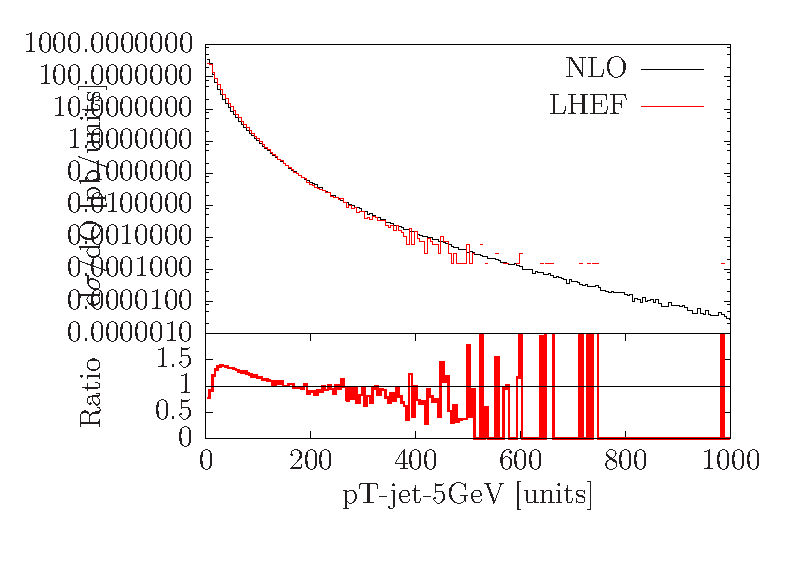
\includegraphics{pT-jet-5GeV}}%
    \gplfronttext
  \end{picture}%
\endgroup
